\chapter{Einleitung und Übersicht}

\section{Einleitung}

Ziel dieser Arbeit ist es, eine mandantefähige Plattform zu konzipieren, zu entwickeln und zu veröffentlichen. Diese soll es Anbietern von Produkten und Services ermöglichen, ihre Drohnen für einen begrenzten Zeitraum oder für bestimmte Aufgaben zur Verfügung zu stellen. Das Ausführen einer Aufgabe soll, bis auf das Beladen der Drohne, komplett automatisiert ablaufen. \\

Sobald ein Kunde eine Bestellung über eine App tätigt, wird automatisch eine Route zu seiner Position berechnet, die über vordefinierte, sichere Zonen führt. Über ein auf der Drohne angebrachtes Smartphone, werden Anweisungen für die Beladung angezeigt. Sobald die Vorbereitungen abgeschlossen sind, bewegt sich die Drohne, mit Hilfe von GPS, entlang der berechneten Route, erfüllt ihre Aufgabe und kehrt wieder zurück. Während der Mission werden laufend Telemetriedaten an den Server geschickt, welcher diese für den Anbieter visualisiert.\\

Project Helin wird als Open Source Software veröffentlicht und kann dann von jedem Interessertien gehostet und weiterentwickelt werden.\\

In der weiteren Dokumentation werden die Anforderungen, die Architektur, die wichtigsten Punkte der Umsetzung sowie der Aufbau eines Anwendungsbeispiels mit zwei echten Drohnen beschrieben.

\section{Ausgangslage}

Alle Multicopter verfügen bereits in der Grundausstattung über einen \Gls{Flight-Controller}, der die Befehle der Fernbedienung in Steuerbefehle für die Motoren übersetzt. Ausserdem nutzen viele Modelle zusätzliche Sensoren (GPS, Beschleunigungsmesser), um autonome Flüge zu ermöglichen und den Copter stabil halten. \\

Um laufend Telemetriedaten zu erhalten und Funktionen steuern zu können, wird in den meisten Fällen über Funk mit dem Copter kommuniziert. Dafür wird ein mobiles Gerät verwendet (Smartphone, Tablet, Notebook) auf dem eine Bodenstationssoftware läuft. Dies ermöglicht die Steuerung in einem Umkreis von ca. 2 km. Zusätzlich können mit Hilfe einer Bodenstationssoftware fixe Routen auf den \Gls{Flight-Controller} gespeichert werden, die dann im Automatikmodus autonom geflogen werden.

\newpage
Dieses bewährte System hat allerdings einige Einschränkungen: 

\begin{itemize}
	\item{Reichweite ist begrenzt}
	\item{Daten der Flüge sind nur für einen Benutzer einsehbar (Lokale Speicherung der Daten)}
	\item{Flugrouten müssen von Hand eingegeben werden}
	\item{Keine zentrale Komponente, auf die andere Systeme (z.B. Bestell-Apps) zugreifen und Aktionen der Drohnen auslösen können}
\end{itemize}

Project Helin soll nun alle diese Einschränkungen aufheben. Damit können Anbieter neue Dienstleistungen erbringen, die nur mit autonomen Flugdrohnen in einer sinnvollen Effizienz möglich sind. Beispielsweise macht es nur in den seltensten Fällen Sinn, Lieferungen mit Drohnen auszuführen, wenn diese von Hand geflogen werden müssen. \\

Bis jetzt gibt es kein vergleichbares offenes System, dass mit Drohnen über das Internet (4G) live kommuniziert und gleichzeitig die Anbindung von zusätzlichen Systemen erlaubt.

\section{Gesetzliche Rahmenbedingungen}
Für den Flug mit Drohnen in der Schweiz gelten die Vorgaben des Bundesamtes für Zivilluftfahrt (BAZL). Die für uns relevanten Punkte umfassen:
\begin{itemize}
	\item{\blockquote{Für den Betrieb von Drohnen und Flugmodellen mit einem Gewicht von über 30 Kilogramm braucht es eine Bewilligung des BAZL.} \cite{drohne-bazl}}
	\item{\blockquote{Über Menschenansammlungen bzw. im Umkreis von 100 Metern von Menschenansammlungen dürfen Drohnen grundsätzlich nicht betrieben werden.} \cite{drohne-bazl}}
	\item{\blockquote{Ein automatisierter Flug (autonomer Betrieb) innerhalb des Sichtbereiches des «Piloten» ist erlaubt, sofern dieser bei Bedarf jederzeit in die Steuerung eingreifen kann.}
	\cite{drohne-bazl}}
\end{itemize}
In anderen Ländern gelten eher schärfere Regelungen, so ist etwa in den Vereinigten Staaten eine Registrierung für Freizeitdrohnen ab 250g erforderlich \cite[]{pwc-drone}. In vielen Ländern werden die gesetzlichen Rahmenbedingungen aktuell angepasst, so dass auch Drohnen ausser Sichtweite betrieben werden können. Zum Beispiel kann in Polen mit einer theoretischen und praktischen Prüfung eine Lizenz erworben werden um Flüge ausser Sichtweite durchzuführen \cite[]{pwc-drone}.\\

Diese Entwicklung zeigt, dass die Zulassung von autonomen Drohnen auch in der Schweiz zukünftig denkbar ist. 

\section{System Kontext}

Project Helin hat drei verschiedene Nutzerarten: Customer (Kunde), Administrator (Anbieter) und Drone-Operator (Drohnen Operator). Diese werden im Kapitel Anforderungen noch genauer beschrieben.\\

In Abbildung \ref{fig:system-context-diagram} sind die externen Schnittstellen, sowie die Aktoren dargestellt. Google OAuth und PayPal werden auf der Customer-App für die Authentifizierung und das Payment eingesetzt. Die 3DR-Service-App wird auf dem Onboard-App benötigt um die Kommunikation mit dem \Gls{Flight-Controller} der Drohne zu ermöglichen. Für die Kartendarstellungen auf der Administrations-Webseite werden von Open Street Map gehostete Karten verwendet.


\begin{figure}[h]
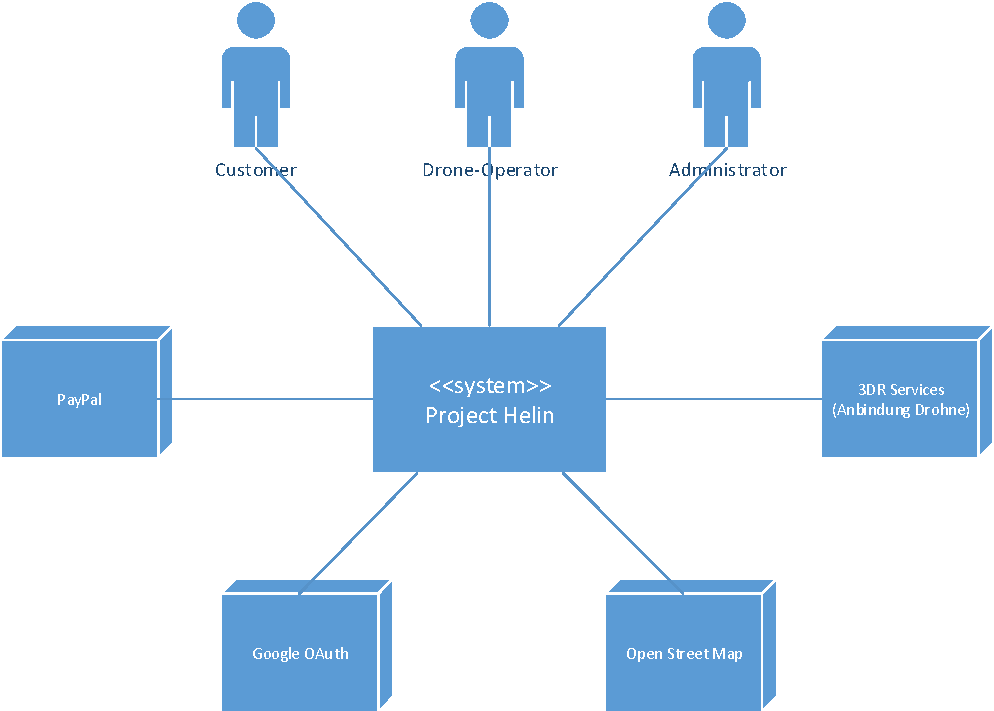
\includegraphics[width=1.0\textwidth]{images/system-context-diagram.pdf}
\caption{System Kontext Diagramm mit externen Schnittstellen }
\label{fig:system-context-diagram}
\end{figure}









